%%% Uncertainity Quantification

\chapter{Optimal Control using Uncertainity Quantification}

\paragraph{Kinetic parameters} are generally empirical constants determined by fitting experimental data to the model, and, hence, are a source of uncertainty within the system. Two methods are discussed here to quantify these uncertainities and thereby perform build a more robust dynamic optimization.

\section{Stochastic Optimal Control using Ito Processes}

From several previous works it has been shown that the dynamic uncertainties
such as the batch reactors\cite{benavides2} and batch distillation,\cite{diwekar}, can be represented using stochastic processes called as the Ito processes.  We characterize the time-dependent uncertainties in the state variables using Ito processes.\\
The advantage lies in the ability to integrate the equations using the principles of stochastic calculus and the use of stochastic maximum principle to solve for the optimal temperature profile. \\
In batch crystallization kinetics, the growth and nucleation expressions have empirical constants shown in Table \ref{Table1}, they can be assumed to follow a Gaussian distribution\cite{yenkie}. By studying the nature of the dynamic uncertainty plots of the process variables and their correlation to Ito processes, it has been observed that the uncertainties can be best modeled with a simple Ito process known as \textbf{Brownian motion} with drift\cite{diwekar,wong}. It can be defined as:
\begin{equation} \label{gen}
dy = a(y,t)dt + b(y,t)dz
\end{equation}
where $dz$ is the increment of the Wiener process equal to $\varepsilon_{t}(\Delta t)^{1/2}$, and a(y,t) and b(y,t) are known functions. The random value $\varepsilon_{t}$  has a unit normal distribution with zero mean
and a standard deviation of 1. To estimate the values of the functions a and b, a generalized method presented by Diwekar\cite{diwekar} has been used.\\
In this work, equation(\ref{gen}) has been used to incorporate the uncertainties into the moment equations which are\cite{yenkie} :
\begin{align}
dy_{1} &= \left[-3\rho k_{v}G(t)(y_{4}+y{8})\right]\Delta t + g_{1}\varepsilon_{1}\sqrt{\Delta t} \\
dy_{2} &= 0 \\
dy_{3} &= (G(t)y_{2})\Delta t +g_{3}\varepsilon_{3}\sqrt{\Delta t} \\
dy_{4} &= (2G(t)y_{3})\Delta t + g_{4}\varepsilon_{4}\sqrt{\Delta t} \\
dy_{5} &= (3G(t)y_{4})\Delta t + g_{5}\varepsilon_{5}\sqrt{\Delta t} \\
dy_{6} &= (B(t))\Delta t + g_{6}\varepsilon_{6}\sqrt{\Delta t} \\
dy_{7} &= (G(t)y_{6})\Delta t + g_{7}\varepsilon_{7}\sqrt{\Delta t} \\
dy_{8} &= (2G(t)y_{7})\Delta t +g_{8}\varepsilon_{8}\sqrt{\Delta t} \\
dy_{9} &= (3G(t)y_{8})\Delta t + g_{9}\varepsilon_{9}\sqrt{\Delta t} \\
\end{align}
$a(y,t)$ in each equation is replaced by the corresponding deterministic function   for the state variable.\\
Here, the $g_{i}$ values represent the variance in the variable for which they are associated. They are calculated by recording the variance of the differences in $y_{i}$, which is divided by the time
interval $\Delta t$, and then the square root of this value is taken.


\paragraph{Objective Function} for the stochastic formulation now becomes :
\begin{equation} \label{objective}
\max_{T} L = \mathbf{E}\left[ \mu_{3}^{s}(t_{f}) - \mu_{3}^{n}(t_{f})\right]
\end{equation}
$\mathbf{E}$ is the expected value of the variable. \\
The \textbf{Active Constraints} and \textbf{Initial Conditions} remain the same as mentioned in Section (\ref{deterministic}).

\subsection{Solution Technique : Stochastic Steepest Ascent Hamiltonian}

The Hamiltonian for this section is modified to incorporate the uncertainities as\cite{yenkie} :
\begin{equation}
H = \sum_{i=1}^{9} \left( z_{i}f_{i} + \omega_{i}\frac{g_{y_{i}}^2}{2} \right)
\end{equation}
$f_{i}$ are the deterministic parts for the eq (5.2-5.11). $\omega_{i}$ is an additional adjoint variable defined to calculate the Hamiltonian for the \textbf{Stochastic Maximum Principle} formulation\cite{ramirez}.  

The \textbf{Algorithm} for the method remains same as mentioned in Section (4.1.1) with minor changes.
\begin{enumerate}
\item  Steps (1-4) are repeated. 
\item The variable θi corresponds to each of the state variable yi and the variable ∮ i corresponds to each of the adjoint variable zi , Ψi corresponding to each ωi respectively.
\item The variable $\theta_{i}$ corresponds to each of the state variable $y_{i}$ and the variable $\phi_{i}$ corresponds to each of the adjoint variable $z_{i}$, $\psi_{i}$ for each $\omega_{i}$ respectively.

\item The Hamiltonian derivative is now calculated at each time step  as :
\begin{align}
&\theta = \frac{dy_{i}}{dT} \quad \phi_{i} = \frac{dz_{i}}{dT} \quad \psi = \frac{d\omega_{i}}{dT} \\
&\frac{dH}{dT} = \sum_{i=1}^{9} \left( \frac{dH}{dy_{i}}\right)\left(	\frac{dy_{i}}{dT} \right) + \sum_{i=1}^{9} \left(\frac{dH}{dz_{i}}\right)\left(\frac{dz_{i}}{dT} \right) + \sum_{i=1}^{9} \left(\frac{dH}{dw_{i}}\right)\left(\frac{dw_{i}}{dT} \right)
\end{align}
\item The convergence criteria and the constraints remain same as the above referenced method.
\end{enumerate} 


\subsection{Results}
The following values were used as the coefficients for uncertainities for the state variables :
\begin{center}
\begin{table}[!h]
\centering
\caption{State Variable Uncertainity Coefficients\cite{yenkie}}
\begin{tabular}{|c|c|}
\hline
Parameters & Values \\
\hline
$g_{1}$ & $2.659\times10^{-5}$ \\
$g_{2}$ & $0$ \\
$g_{3}$ & $25.882$ \\
$g_{4}$ & $1.517\times10^{4}$ \\ 
$g_{5}$ & $6.57\times10^{6}$ \\
$g_{6}$ & $0.5486$ \\
$g_{7}$ & $25.9$\\
$g_{8}$ & $1382.34$ \\
$g_{9}$ & $8.753\times10^{4}$ \\
\hline
\end{tabular}

\label{Table2}
\end{table}
\end{center}

\begin{itemize}
\item The stochastic differential equations are integrated using stochastic calculus through \textbf{SDE Tools} Library available in \textbf{Matlab}.A strong Taylor approximation from the \textbf{Euler Maruyama} scheme has been used to integrate the equations which has an order of convergence of 0.5. 
\end{itemize}
The following profiles were obtained as a result :
\begin{figure}[h!] 

\begin{center}
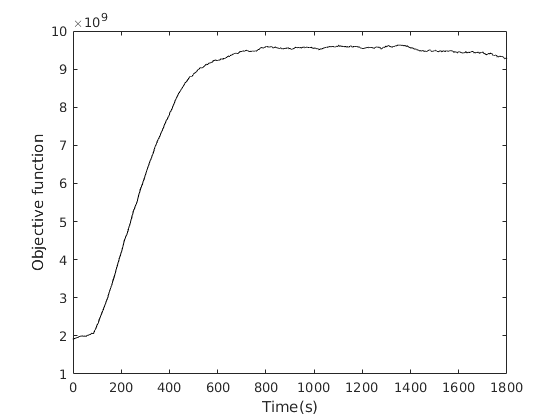
\includegraphics[width=4in]{Sobj.png}
\end{center}
\caption{Objective Function ($\mathbf{E}\left[\mu_{3}^{s}(t) - \mu_{3}^{n}(t)\right]$)}
\end{figure}
\begin{figure}[h!] 

\begin{center}
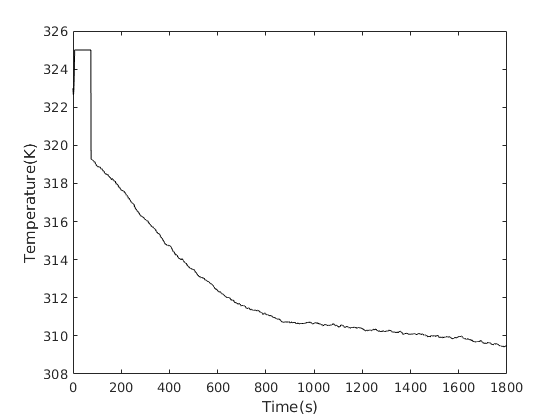
\includegraphics[width=4in]{Stemp.png}
\end{center}
\caption{The cooling profile for the controlled variable T(t) obtained at the final iteration}
\end{figure}

\begin{figure}[h!] 

\begin{center}
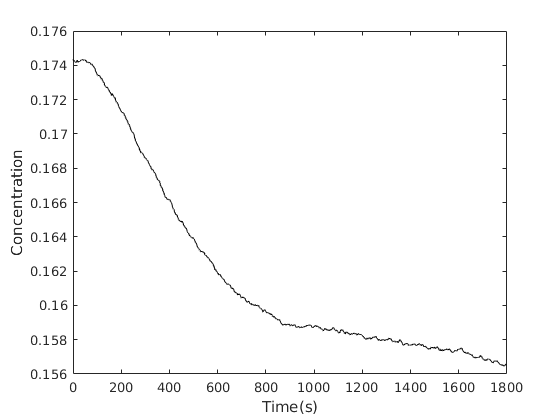
\includegraphics[width=4in]{Sconc.png}
\end{center}
\caption{Concentration Profile as obtained}
\end{figure}
\clearpage

\section{Stochastic Optimal Control using Polynomial Chaos Expansions}

\subsection{Introduction}
A Polynomial Chaos Expansion (PCE) describes a random process as a spectral expansion of random variables($\theta_{i}$), using orthogonal basis functions, $\Phi_{i}$ (Ghanem and Spanos, 1990,Ghanem and Spanos, 1997). For example, any second-order (finite variance) random process $y^{d}$, can be described using a PCE as follows:
\begin{equation}
y^{d} = a_{0}^{d}\phi_{0} + \sum_{i_{1}=1}^{\infty} a_{i_{1}}^{d}\phi_{1}(\theta_{i_{i1}}) + \sum_{i_{1}=1}^{\infty}\sum_{i_{2}=1}^{i_{1}} a_{i_{1}i_{2}}^d\phi_{2}(\theta_{i_{1}},\theta_{i_{2}})
\end{equation}
where $a_{i_{1}}^d$  are deterministic coefficients for each term in the expansion. The number of independent sources of random variables $(\theta_{i_{1}}, \theta_{i_{2}})$, generally defines the dimensionality, $n_{0}$. For practical application these expansions can be
truncated to a finite number of terms. Then the maximum polynomial order for the basis function, q needs to be defined.
The number of terms now become $P_{PCE} = \frac{(n_{0}+q)!}{n_{0}!q!} -1 $. \\
Using these notations a truncated PCE expansion can be represented as follows:
\begin{equation}
y^{d} \approx \sum_{i=1}^{P_{PCE}} a_{i}^{d}\phi_{\theta}
\end{equation}

The orthogonality property of the basis functions($\phi_{i}$) is used for the  calculation of the coefficients when propagating uncertainty from the input random variables$(\theta_{i_{1}}, \theta_{i_{2}})$, to the output random
variables ($y^{d}$).\\
The choice of the basis functions $\phi_{i}$ depends on the type of stochastic distribution to be represented, i.e. normal or uniform. In our case the parameters follow a Gaussian distribution\cite{yenkie}, which uses Hermite Polynomials to describe the probability distribution in the least number of terms.\\
Thus, given a process model with uncertain output, $y = X(x,\lambda)$, where $x$ is the uncertain input and $\lambda$ is the uncertain parameter, the aim is to quantify uncertainty in $y(\theta)$ from $x(\theta), \lambda(\theta)$ using the process model. Then the first step is to construct PCE’s of $x(\theta)$, and $\lambda(\theta)$, by determining their PCE coefficients $x_{i}$ and $\lambda_{i}$.
\begin{align}
&x(\theta) = \sum_{i=1}^{P_{PCE}} x_{i}\phi(\theta)
&\lambda(\theta) = \sum_{i=1}^{P_{PCE}} \lambda_{i}\phi(\theta)
\end{align}
\begin{equation}
&x_{i} = \frac{\int x\phi_{i}(\theta)g(\theta) d\theta}{\left\langle \phi^{2}_{i}\right\rangle } \quad
&\lambda_{i} = \frac{\int \lambda\phi_{i}(\theta)g(\theta) d\theta}{\left\langle \phi^{2}_{i}\right\rangle }
\end{equachaospytion}
where $g(\theta)$ is probability distribution function (pdf) of $\theta$. 
The next step is to develop PCE for $y(\theta)$ from  $x(\theta)$, and $\lambda(\theta)$, which can be done by evaluating the
inner product of $y(\theta)$ with each basis functions $\phi_{i}$ to determine the ith- PCE coefficient.
\begin{equation}
y_{i} = \frac{\left\langle f(x,\lambda)\phi_{i} \right\rangle }{\left\langle \phi^{2}_{i} \right\rangle }
\end{equation}
Evaluating the inner product $\left\langle y\phi_{i} \right\rangle $, requires computation of multi-dimensional integrals which can be performed by one of two approaches referred to as \textbf{non-intrusive} and \textbf{intrusive}.\\
The work under consideration here uses a non-intrusive approach. The model $y=X(x,\lambda)$ is represented by the modelling equations of Section(\ref{modeleq}). $x$ are the state variables and $\lambda$'s are the kinetic parameters. 
\subsection{Solving a system of O.D.E using P.C.E approach}

The generalized polynomial chaos framework is widely used to propagate the time invariant stochastic uncertainties through the nonlinear system dynamics and has been proved to be more efficient than traditional control methods. Thus this speciality has been exploited in our case to model the seeded batch crystallizer.\\
The uncertainities in the model are due to the following kinetic parameters :

\begin{center}
\begin{table}[!h]
\centering
\caption{Kinetic Parameter Uncertainities\cite{hu,shi,paeng}}
\begin{tabular}{|c|c|c|}
\hline
Parameters & Experimental Values & Range of Values\\
\hline
\multicolumn{3}{|c|}{Growth Kinetics} \\
\hline
$k_{g}$ & $1.44\times10^{8} \mu m s^{-1}$ & $1.368 - 1.512\times10^{8} $\\
$E_{g}/R$ & $4859K$ & $4606.15-5101.95$\\
$g$ & $1.5$ & $1.425-1.575$\\
\hline
\multicolumn{3}{|c|}{Nucleation Kinetics} \\
\hline
$k_{b}$ & $285 (s \mu m^{3})^{-1}$ & $270.75-299.25$\\ 
$E_{b}/R$ & $7517K$ & $7141.15-7892.85$\\
$b$ & $1.45$ & $1.3775-1.5225$\\
\hline
\end{tabular}

\label{Table3}
\end{table}
\end{center}
\paragraph{Non-Intrusive Approach} estimates the integrals based on N samples of the whole space of basis functions. \textbf{Intrusive Appraoch} on the other hand, solves it analytically using the basis functions but requires the system to be separable in terms of uncertain parameters and inputs(polynomial-in-states representation). \\
Thus, Point Collocation Approach(Non-Intrusive) is selected for modeling the uncertainities. 

\paragraph{Algorithm}
\begin{enumerate}
\item The process model consists of 6 uncertainities which computationally prohibits the evaluation. Thus, an approximation of $n_{0} = 2$ is taken by employing a joint distribution of the parameters.
\item Samples are generated using the distribution using Gaussian Quadrature Scheme.
\item The function is evaluated at each of these samples to evalute the integrals numerically to determine the PCE coefficients.
\item At each sample, optimization of the model is performed using the Determinstic Approach explained in Section(\ref{deterministic}).
\item The convergence criteria and the constraints remain same as the above referenced method.
\end{enumerate}


\paragraph{Objective Function} is given by eq \ref{objective}. 


\subsection{Results}

\begin{itemize}
\item The method was implemented in pyhton using the \textbf{chaospy} library\cite{chaospy} for Polynomial Chaos Expnasions. 
\end{itemize}
The following profiles were obtained : 

\begin{figure}[h!] 

\begin{center}
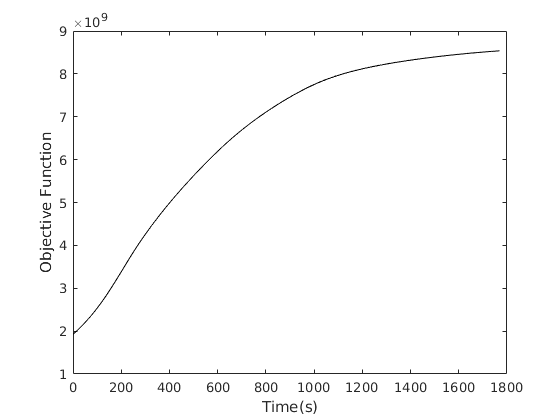
\includegraphics[width=4in]{PCEobj.png}
\end{center}
\caption{Objective Function ($\mathbf{E}\left[\mu_{3}^{s}(t) - \mu_{3}^{n}(t)\right]$)}
\end{figure}
\begin{figure}[h!] 

\begin{center}
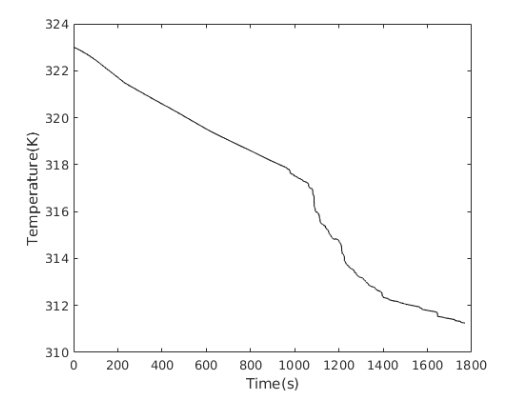
\includegraphics[width=4in]{PCETemp2.png}
\end{center}
\caption{The cooling profile for the controlled variable T(t) obtained at the final iteration}
\end{figure}

\begin{figure}[h!] 

\begin{center}
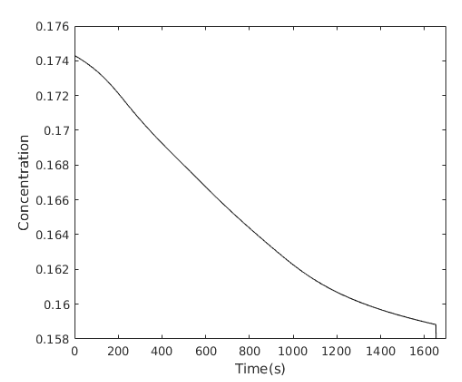
\includegraphics[width=4in]{PCEConc.png}
\end{center}
\caption{The concentration profile as obtained.}
\end{figure}
\clearpage

\section{Conclusions}
\begin{itemize}
\item The same process was optimized using 3 different methods of Optimization. This achieves the aim of maximising the volume of the product obtained. 
\item The Temperature profile for all the 3 cases was obtained as a decreasing one and thus follows the principle of batch cooling crystallization. 
\item Polynomial Chaos Expansions, when applied to crystallization performs at par with the existing methods in optimizing the process by efficiently incorporating uncertainities. 
\item After comparing the final values of the objective functions($\mu_{3}^{s}-\mu_{3}^{n}$) the following values were obtained : 
\begin{enumerate}
\item Deterministic : $ 9.153 \times 10^{9}$
\item Expected value for Stochastic involving Ito Processes : $8.978 \times 10^{9}$
\item Expected value for Stochastic case involving PCE : $8.64 \times 10^{9}$
\end{enumerate}
\end{itemize}